\documentclass[9pt,twocolumn]{extarticle}

\usepackage[a4paper,margin=1.6cm,columnsep=0.6cm]{geometry}
\usepackage[utf8]{inputenc}
\usepackage[T1]{fontenc}
\usepackage[brazil]{babel}
\usepackage{graphicx}
\usepackage{amsmath}
\usepackage{amssymb}
\usepackage{booktabs}
\usepackage{titlesec}
\usepackage{times}
\usepackage[hidelinks]{hyperref}
\usepackage{caption}

\captionsetup{font=footnotesize, labelfont=bf, skip=2pt}
\titlespacing*{\section}{0pt}{6pt}{3pt}
\titlespacing*{\subsection}{0pt}{4pt}{2pt}
\setlength{\parskip}{0pt}
\setlength{\abovedisplayskip}{3pt}
\setlength{\belowdisplayskip}{3pt}

\pagestyle{empty}

\title{\vspace{-1.2em}\textbf{\large Edição de Atributos Faciais com Preservação de Identidade via Difusão Latente e CFG Composável}\vspace{-0.8em}}
\author{\footnotesize Lucas B. \\[-0.3em] \footnotesize \texttt{lucasbbarcel@gmail.com}}
\date{}

\begin{document}
\maketitle
\vspace{-2.2em}

\begin{abstract}
\footnotesize
Apresentamos um modelo de difusão latente (LDM) para edição de atributos faciais do CelebA que preserva a identidade da pessoa fotografada. Identidade (ArcFace/CLIP) e atributos (40 rótulos binários) são tratados como condicionantes independentes combinados por \emph{Classifier-Free Guidance} (CFG) composável de três termos, evitando as limitações de \emph{Classifier Guidance} (CG) exploradas anteriormente. Uma correção adicional --- usar, como referência de identidade, uma foto \emph{diferente} da mesma pessoa --- elimina o vazamento de expressão que impedia a edição de atributos ligados à expressão facial.
\end{abstract}

\section{Introdução}
O objetivo do projeto é, dada uma foto de uma pessoa, gerar uma nova imagem que preserve sua identidade mas edite atributos faciais escolhidos (sorriso, óculos, calvície etc., conforme os 40 rótulos do CelebA). O desafio central é conciliar dois condicionantes de natureza distinta --- uma identidade contínua (\emph{embedding}) e atributos binários discretos --- sem que um interfira na controlabilidade do outro.

\section{Método}

\subsection{Pipeline de dados}
As imagens do CelebA (recorte nativo $178\times218$, redimensionado para $256\times256$) são codificadas por um VAE congelado (estilo Stable Diffusion, $\mathrm{latent\_dim}=4$) em um cache de latentes, evitando recomputar o encoder a cada época. Um segundo cache armazena, por imagem, o \emph{embedding} ArcFace (identidade, 512-d) e os tokens CLIP ViT-B/32 (aparência). Como o algoritmo de alinhamento original do CelebA nunca foi publicado, foi necessário reconstruir empiricamente o alinhamento nativo do dataset a partir da média dos 5 pontos faciais fornecidos, validando que o procedimento reprojeta corretamente uma imagem perturbada (rotação/deslocamento) de volta ao enquadramento esperado pelo VAE e pelos encoders (Figura~\ref{fig:align}).

\begin{figure}[t]
\centering
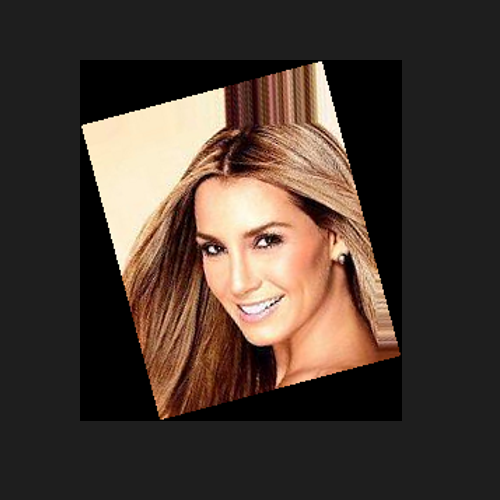
\includegraphics[width=0.46\linewidth]{figures/perturbed.png}\hfill
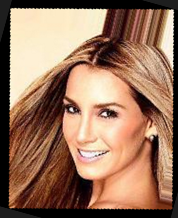
\includegraphics[width=0.46\linewidth]{figures/corrected.png}
\caption{Robustez do alinhamento: entrada perturbada (esq.) corrigida de volta à convenção nativa do CelebA (dir.), usada por VAE, ArcFace e classificador de atributos.}
\label{fig:align}
\end{figure}

\subsection{Arquitetura}
A Figura~\ref{fig:arch} resume a inferência. Uma foto de referência gera \emph{tokens} de identidade via ArcFace (e, opcionalmente, CLIP); os atributos-alvo geram \emph{tokens} via um \texttt{AttributeEmbedder} (\emph{embedding} binário por atributo). Os dois conjuntos de tokens são concatenados em um único contexto, consumido por cross-attention em uma U-Net latente ($32\times32\times4$) que estima o ruído a cada passo reverso; o latente final é decodificado pelo VAE.

\begin{figure}[t]
\centering
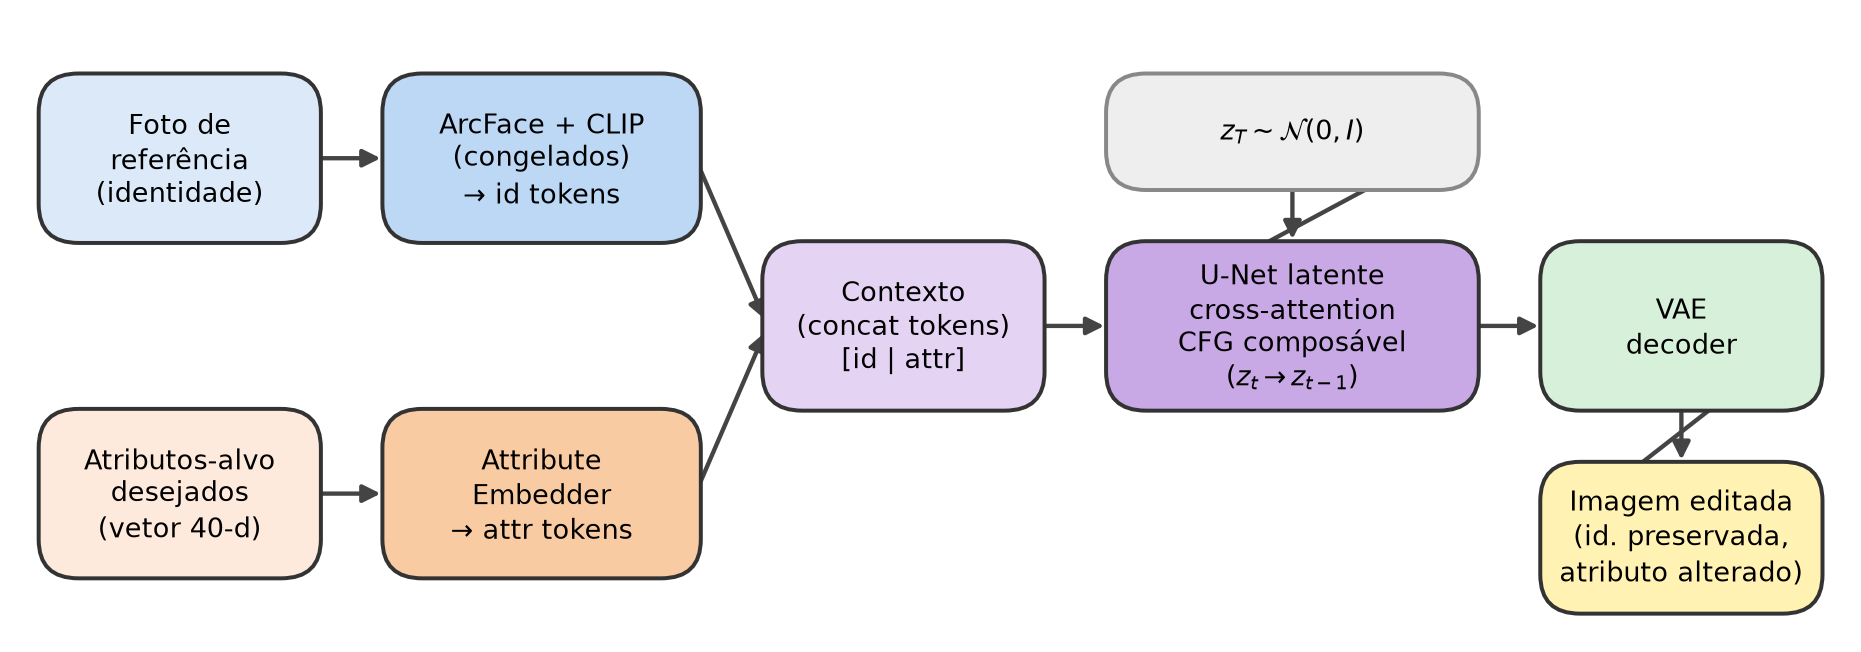
\includegraphics[width=\linewidth]{figures/architecture.png}
\caption{Pipeline de inferência: identidade e atributos são condicionantes independentes, concatenados no contexto de cross-attention da U-Net.}
\label{fig:arch}
\end{figure}

\subsection{De Classifier Guidance para CFG composável}
A arquitetura originalmente combinava CFG (identidade) com \emph{Classifier Guidance} (CG) --- um classificador sobre o latente ruidoso $z_t$ guiando a amostra via $\nabla_{z_t}\log p(y\mid z_t)$. Essa abordagem (\texttt{train\_mixed\_guidance*.py}) foi explorada e descartada por três motivos estruturais: (i) a sigmoid do classificador multi-rótulo satura, colapsando o gradiente quando a predição já é confiante; (ii) o termo somava os 40 atributos, diluindo o sinal do atributo que de fato se deseja editar; (iii) em $t$ alto o latente é quase ruído puro (classificador aprende só o prior) e em $t$ baixo restam poucos passos úteis para editar --- janela estreita.

Adotamos então \emph{Composable Diffusion} (Liu et al., ECCV 2022): identidade e atributo tornam-se dois condicionantes independentes, cada um com seu próprio \emph{dropout} de CFG sorteado por amostra (10\% zera só id, 10\% só attr, 10\% zera ambos, 70\% mantém ambos), e a amostragem combina três \emph{forward passes} da U-Net:
\begin{equation}
\begin{aligned}
\epsilon = {} & \epsilon(\varnothing,\varnothing) + s_{id}\big[\epsilon(\mathrm{id},\varnothing) - \epsilon(\varnothing,\varnothing)\big] \\
& + s_{attr}\big[\epsilon(\mathrm{id},\mathrm{attr}) - \epsilon(\mathrm{id},\varnothing)\big]
\end{aligned}
\label{eq:composable}
\end{equation}
O segundo termo usa $\epsilon(\mathrm{id},\varnothing)$ como base (não $\epsilon(\varnothing,\varnothing)$): mede o quanto o atributo desloca a predição \emph{dada} a identidade já aplicada, tornando os dois termos aproximadamente ortogonais e cada escala ($s_{id}$, $s_{attr}$) independentemente ajustável.

\subsection{Referência de identidade pareada}
Um segundo problema surgiu ao usar CLIP junto do ArcFace: quando a foto de referência é a própria imagem-alvo do \emph{denoising}, o CLIP enxerga a expressão exata que o modelo precisa gerar, e nenhum valor de $s_{attr}$ conseguia sobrepor esse vazamento (ex.: forçar \texttt{Smiling=1} não fazia efeito). A correção (\texttt{train\_cfg\_composable\_paired.py}, método final adotado) usa como referência uma foto \emph{diferente} da mesma identidade, via \texttt{identity\_CelebA.txt} --- no CelebA, identidades têm em média $\sim$20 fotos e 91\% das identidades com $\ge2$ fotos variam no atributo \texttt{Smiling}, garantindo que a maioria dos lotes de treino veja referência e alvo com expressões distintas.

\section{Configuração experimental}
Treinamos com AdamW ($\mathrm{lr}=3\times10^{-4}$, \emph{warmup} linear de 10 épocas seguido de \emph{cosine annealing}), \emph{batch size} 64, precisão mista (AMP) e \emph{EMA} dos pesos, em regime multi-GPU (DDP). A avaliação qualitativa periódica gera, para o mesmo conjunto fixo de referências, duas grades de amostras via DDIM (50 passos): atributos originais e atributos com \texttt{Smiling} forçado a 1 --- teste direto de que a edição funciona sem depender do CLIP. FID contra o conjunto de validação é calculado periodicamente (a partir de uma época mínima, para não desperdiçar tempo em épocas iniciais não informativas) como métrica complementar de fidelidade. Os resultados quantitativos finais do treino pareado ainda estão em coleta; o protocolo acima é o mesmo usado para comparar as variantes \texttt{clip\_arcface} e \texttt{arcface\_only} do encoder de identidade.

\section{Conclusão e trabalhos futuros}
A migração de \emph{Classifier Guidance} para CFG composável, somada ao pareamento da referência de identidade, resolve estruturalmente o vazamento que impedia a edição de atributos ligados à expressão. Direções futuras incluem: cross-attention dedicada por condicionante (estilo IP-Adapter), em vez de concatenar tokens em um único cross-attention; modulação tipo adaLN-Zero/FiLM para os atributos, atuando em todos os blocos da U-Net (não só nas resoluções com cross-attention); e um terceiro ramo independente de CFG que separe ArcFace (identidade pura) de CLIP (aparência/estilo), permitindo zerar a contribuição do CLIP em edições estruturais (ex.: \texttt{Bald}) sem perder identidade.

\end{document}
